\documentclass[lang=en,mode=geye,device=normal,color=blue,14pt]{elegantnote}
\usepackage{amsmath,amssymb}
\usepackage{bbm}
\usepackage{tcolorbox}
\usepackage{graphicx}
\usepackage{booktabs}
 \usepackage{subfigure}
\DeclareMathOperator*{\E}{\mathbb{E}}
\DeclareMathOperator*{\1}{\mathbbm{1}}
\DeclareMathOperator*{\R}{\mathbbm{R}}
\DeclareMathOperator*{\argmax}{arg\,max}
\DeclareMathOperator*{\argmin}{arg\,min}

\title{Note: Reinforcement Learning - An Introduction}

\author{Yanqing Wu}
\institute{Viwistar Robotics}

% \version{0.1.0}
\date{\today}

\begin{document}
\maketitle

\newpage

\section{Chap 1: Introduction}
\subsection{Reinforcement Learning}

RL is learning what to do, so as to maximize a numerical reward signal.

RL means taking optimal action with \textbf{long term} results or \textbf{cumulative rewards} in mind.

Two most important distinguishing features of RL: trial-and-error search and delayed reward.

RL methods generally incorporate 3 aspects: sensation, action and goal.

\begin{definition}
\textbf{Supervised Learning} is learning from a training set of labeled examples provided by a knowledgable external supervisor.
\end{definition}

\begin{itemize}
	\item Example: a description of a situation
	\item Label: a specification of the correct action the system should take in a situation, which is often to identify a category to which the situation belongs
	\item Object of Supervised Learning: for the system to extrapolate (generalize) its responses s.t. it acts correctly in unseen situations
	\item Con: inadequate for learning from interaction, because it is (often) impractical to obtain examples of desired behavior that are both correct and representative of all the situations in which the agent has to act
\end{itemize}

\begin{definition}
\textbf{Unsupervised Learning} is about finding structure hidden in collections of unlabeled data.
\end{definition}
RL is trying to maximize a reward signal, while Unsupervised Learning is trying to find hidden structure

Key feature 1: the exploration-exploitation dilemma is one of RL's challenges.
Exploitation: to obtain reward from experienced.
Exploration: to find better actions.

Key feature 2: RL explicitly considers the whole problem of a goal-directed agent interacting with an uncertain environment.

\subsection{Examples}
\subsection{Elements of RL}

Four main subelements of a RL system: a \textit{policy}, a \textit{reward signal}, a \textit{value function}, and a \textit{model} of the environment.

\begin{definition}
\textbf{Policy}, defines the learning agent's way of behaving at a given time.
\end{definition}

A policy is a mapping from perceived states of the environment, to actions to be taken, when in those states.
A policy may be a simple function or a lookup table, or complex computation (e.g. a search process).
Policies may be stochastic, specifying probabilities for each action.

\begin{definition}
\textbf{Reward signal}, defines the goal of a RL problem.
\end{definition}

On each timestep, the environment sends a single number (i.e. \textit{reward}) to the RL agent. The agent's only objective is to maximize the total reward it receives over the long run.

\begin{definition}
\textbf{Value function}, specifies what is good in the long run.
\end{definition}

The \textit{value} of a state is the total amount of reward an agent can expect to acumulate over the future, starting from that state.

\textit{Rewards} determine the immediate desirability of states, \textit{values} determines the long-term desirability of states.

State Value function = Expected Return = Discounted sum of all rewards

\begin{definition}
\textbf{Model}, mimics the behavior of the environment.
\end{definition}

Models are used for \textit{planning}.
Model-based methods: use models and planning to solve RL problems.
Model-free methods: explicitly trial-and-error learner (almost the opposite of planning).

Modern RL spans the spectrum from low-level, trial-and-error learning to high-level, deliberative planning.

\subsection{Limitations and Scope}
\subsection{An Extended Example: Tic-Tac-Toe}
Minimax algorithm \cite{wiki_minimax} (from game theory).

Classical optimization methods for sequential decision problems (e.g. dynamic programming). We need to estimate an approximate opponent model so to use dynamic programming; in such case, this is similar to RL methods.

During playing, we need to adjust the values of the states as to make more accuracte estimates of the probabilities of winning. The current value of the earlier state is updated to be closer to the value of the later state. This can be done by moving the earlier state's value a fraction of the way toward the value of the later state.

\begin{equation}
V(S_t) \leftarrow V(S_t) + \alpha[V(S_{t+1}) - V(S_t)]
\end{equation}

$S_t$, the state before a move.
$S_{t+1}$, the state after the move.
$V(S_t)$, the update to the estimated value of $S_t$.
$\alpha$, step-size parameter, a small positive fraction, influences the rate of learning.

This update rule is an example of a temporal-difference (TD) learning method. TD means the changes are based on a difference between estimates at two consecutive times.

If $\alpha$ is reduced properly over time, then this method converges (for any fixed opponent, it converges to the true probabilities of winning for each state); if $\alpha$ is not reduced to zero over time, then the agent ``also plays well against opponents that slowly change their way of playing'' (?). My understanding is that, there must have some changes, whether the parameter or the opponent model.

\textbf{Evolutionary methods vs. Value Function methods.} Evolutionary methods ignores what happens during the games, and only the final outcome of each game is used (e.g. all of its behavior in a winning game is given credit). In contrast, value function methods evaluate individual states.

In this example, learning started with no prior knowledge except the rules of the game. In reality, prior information can be incorporated into RL in many ways for efficient learning.
RL can be used when we have access to true state, or where some states are hidden, or when different states appear to be the same to the learner.

The player need a model of the game to see the result states in response to actions. While model-free systems cannot know how their environments will change in response to actions.
Model-free methods are building blocks for model-based methods.
Sometimes, it is difficult to construct an accuract environment model, thus model-based methods cannot be used in such cases.

\subsection{Summary}

RL is a computational approach to understanding and automating goal-directed learning and decision making.
It is distinguished from other computational approaches by its emphasis on learning by an agent from direct \textbf{interaction} with its environment, without requiring exemplary supervision or complete models of the environment.

RL uses the formal framework of Markov decision processes (MDP) to defined the interaction between a learning agent and its environment in terms of states, actions, and rewards.

The concepts of value and value function are key to most of the RL methods in this book.
The authors believe that value functions are critical for efficient search in policy space.
The use of value functions distinguishes RL methods from evolutionary methods.

\subsection{Early History of RL}

Three threads: 
1. learning by trial and error, originated in the psychology of animal learning. Time from 1850s to early 1980s' revival of RL;
2. optimal control problem and its solution using value functions and dynamic programming. This thread did not involve learning;
3. temporal-difference methods.
These 3 threads came together in late 1980s.
The TD and optimal control threads were fully brought together in 1989 with Chris Watkin's development of Q-learning.

The essential idea of trial-and-error learning: `the drive to achieve some result from the environment, to control the environment toward desired ends and away from undesired ends.'

TD learning methods are driven by the difference between temporally successive estimates of the same quantity.

The authors developed a method for using TD learning + trial-and-error learning, known as the \textit{actor-critic architecture}.

\newpage
\textbf{Part I: Tabular Solution Methods}

Algorithms in this part are described in simplest forms: the state space and action space are small enough for the approximate value functions to be represented as arrays/tables.
In this case, the methods can (often) find exact solutions (i.e. optimal value function and optimal policy).
Algorithms in next part can only find approximate solutions but can be applied to much larger problems.

\textbf{Bandit problems}, RL problem with only a single state. Chap. 2 describes general problem formulation (finite MDP) and its main ideas (including Bellman equations and value functions).

Three fundamental classes of methods for solving MDP problems: dynamic programming, Monte Carlo methods and TD learning.
\begin{itemize}
\item DP: well developed, but require a complete and accurate model of the environment
\item MC: no model needed, but not good for incremental computation
\item TD: no model needed and fully incremental, but are complex
\end{itemize}

\section{Chap. 2 Multi-armed Bandits}
\begin{itemize}
\item Evaluative: feedback depends solely on the taken action
\item Instructive: feedback is independent of the taken action
\item Nonassociative setting: no learning involved in more than one situation; no need to associate different actions with different situations/states
\item Associative setting: the best action depends on the situation
\end{itemize}

\subsection{A k-armed Bandit Problem}

\textit{k-armed badit problem}:
You choose one option (action) from \textit{k} different options (actions). The probability of choosing each option (action) is stationary. For each choice, you receive a (probably distinct) numerical reward. Your objective is to maximize the expected total reward over \textit{j} option selections (time steps).

For now, let us define that

\textit{Value}: the expected/mean reward of a taken action.
$A_t$: action selected on time step $t$
$R_t$: corresponding reward of $A_t$
$q_{*}(a)$: the (true) value of an arbitrary action $a$ (i.e. the expected reward given $a$ is selected) $$q_{*}(a) \doteq \E[R_t|A_t=a]$$

If we know each action values, then solving the \textit{k}-armed bandit problem would be always select the action with highest $value$.
If we don't know the action values, then we can estimate them. Let

$Q_t(a)$: the \textit{estimated} value of action $a$ at time step $t$.

Our goal is to have $Q_t(a)$ to be as close to $q_*(a)$ as possible.

\begin{definition}
\textbf{Greedy actions}, action(s) with highest estimated value.
\end{definition}
\textit{exploiting}: select greedy action(s).
\textit{exploring}: select non-greedy action(s); this may improve the estimate value of non-greedy actions.

\subsection{Action-value Methods}

\begin{definition}
\textbf{Action-value Methods}, a.k.a Q function, methods for estimating the values of actions, and using the estimates to select actions.
\end{definition}

`Q' means the \textbf{quality} of an action.

Let see a simple action-value method: \textit{sample-average method}, averaging the received rewards.

$$ Q_t(a) \doteq \frac{\sum_{i=1}^{t-1}R_i \cdot \1_{A_{i=a}}}{\sum_{i=1}^{t-1}\1_{A_{i=a}}}$$

\begin{itemize}
	\item $\1$: return 1 if predicate is true, otherwise 0
	\item in the case when denominator is 0 (which makes the fraction mathematically undefined), $Q_t(a)$ is set as default value (e.g. 0)
	\item in the case when denominator $\rightarrow \infty$, by the Law of Large Numbers, $Q_t(a)$ converges to $q_*(a)$
\end{itemize}

\begin{definition}
\textbf{Greedy action selection}, If there are more than one greedy action, select one of them arbitrarily.
$$ A_t \doteq \argmax_{a} Q_t(a) $$
\end{definition}

\begin{definition}
\textbf{$\varepsilon$-greedy action selection} with probability $\varepsilon$, select an action randomly; with probability $1-\varepsilon$, select a greedy action
\end{definition}

\subsection{The 10-armed Testbed}

For Exercise 2.2, note that we should first convert the sequence of actions and rewards to $Q_t(a)$, then we can decide whether the selection is greedy or exploration based on the definition of $\varepsilon$-greedy action selection.

\subsection{Incremental Implementation}

Recall that estimated action value $Q_n$, using sample-average method, is calculated as:
$$ Q_n \doteq \frac{R_1 + \cdots + R_{n-1}}{n-1} $$

We don't want to waste memory and computational resource for each new reward.
Intuitively, to save memory, we can simplify the equation by first reconstruct the previous estimated action value $Q_{n-1}$ and then evaluate $Q_n$ with the new reward $R_n$.
Therefore,
$$ Q_{n+1} = \frac{Q_n \cdot (n-1) + R_n}{n} = \frac{Q_n \cdot n - Q_n + R_n}{n} = Q_n + \frac{1}{n}[R_n - Q_n] $$

The form $Q_{n+1} = Q_n + \frac{1}{n}[R_n - Q_n]$ is an important form occurs in this book. The general form is
$$ NewEstimate \leftarrow OldEstiamt + StepSize\underbrace{[Target - OldEstimate]}_{error} $$

% \begin{tcolorbox}[width=\textwidth,colback={grey},title={A simple bandit algorithm},colbacktitle=black,coltitle=white]}
\begin{tcolorbox}[width=\textwidth,title={A simple bandit algorithm}]
	\begin{align*}
	   & \text{Initialize, for a = 1 to }k: \\
	   & \quad Q(a) \leftarrow 0 \\
	   & \quad N(a) \leftarrow 0 \\
	   & \text{Loop forever: }\\
	   & \quad A \leftarrow \left\{
	    \begin{array}{ll}
	        \argmax_x Q(a) & \text{with prob. } 1 - \varepsilon \text{ (breaking ties randomly) }\\
	        \text{a random action} & \text{with prob. } \varepsilon
	    \end{array}
	\right. \\
	   & \quad R \leftarrow bandit(A) \\
	   & \quad N(A) \leftarrow N(A) + 1 \\
	   & \quad Q(A) \leftarrow Q(A) + \frac{1}{N(A)}[R-Q(A)]
	\end{align*}
\end{tcolorbox}

\subsection{Tacking a Nonstationary Problem}

In previous section, the reward probability distribution is stationary (i.e. doesn't change over time).
For nonstatoinary cases, let say we give more weight to recent rewards than to `long-past' rewards; for doing so, one popular way is to use a constant $\alpha$ (step size).

Not all choices of $\alpha_n(a)$ guarantee convergence.
In \textit{stochastic approximation theory}, two conditions required to assure convergence with probability 1:

$$ \sum_{n=1}^\infty \alpha_n(a) = \infty $$
$$ \sum_{n=1}^\infty \alpha_n^2(a) < \infty $$

The 1st condition is required to guarantee that the steps are large enough to eventually overcome any initial conditions or random fluctuations.
The 2nd condition is required to guarantee that the steps eventually become small enough to assure convergence.

Therefore, in sample-average method, $\alpha_n(a) = \frac{1}{n}$ converages, but a constant step-size parameter $\alpha_n(a)=\alpha$ does not converge.

Note that sequences of $\alpha$ that meet the conditions often converge very slowly and often need considerable tunning.
These sequences of $\alpha$ often used in theoretical work, and are seldom used in real-world application.

\subsection{Optimistic Initial Values}

Higher (more optimistic) initial values may result in better performance. More optimistic initial values ($Q_i(a)$) encourages more exploration.
This may only work well on stationary problems; as in nonstationary problems, the drive for exploration is inherently temporary.

\subsection{Upper-Confidence-Bound Action Selection}

In $\varepsilon$-greedy action selection, it is not ideal to just randomly select actions; instead, we want to select among the non-greedy actions according to their potential for actually being optimal. Such taking into account both (1) how close their estimates are to being maximal, and (2) the uncertainties in those estimates.

\begin{definition}
Upper-Confidence-Bound (UCB) Action Selection

\[
A_t \doteq \argmax_a \bigg[ Q_t(a) + c\sqrt{\frac{\text{ln }t}{N_t(a)}} \bigg]
\]
\end{definition}
$N_t(a)$, denotes the number of times that action $a$ has been selected prior to time $t$. If $N_t(a)=0$, then $a$ is considered to be a maximizing action.
$c$, $c > 0$ (confidence level) controlsthe degree of exploration

The idea os UCB action selection is that the square-root term is a measure of the uncertainty/variance in the estimate of $a$'s value.
Each time $a$ is selected, the uncertainty is (presumably) reduced as $N_t(a)$ increments.
Each time a non-$a$ is selected, $t$ increments but $N_t(a)$ doesn't, thus the uncertainty estimate increases.
All actions will eventually be selected, but actions with lower value estimates or that have been frequently selected, will be selected with decreasing frequency over time.

UCB is useful in bandit problems, but is (usually) not practical in general RL settings. It is difficult to deal with (1) nonstationary problems, and (2) large state spaces.

\subsection{Gradient Bandit Algorithms}
We have considered methods that (1) estimate actions values; (2) select actions based on estimations.
We now consider a new approach for action selection: learning a numerical \textit{preference} for each action \textit{a}, which we denote $H_t(a) \in \R$.
The larger the preference, the more often that action is taken, but the preference has no interpretation regarding rewards.
Only the \textbf{relative} preference of one action over another is important.
The action probabilities is determined by \textit{soft-max distribution}.

\[
P(A_t=a) \doteq \frac{e^{H_t(a)}}{\sum_{b=1}^k e^{H_t(b)}} \doteq \pi_t(a)
\]

$\pi_t(a)$ is the probability of taking action $a$ at time $t$. The initial probability are the same for all actions.

There is a natural learning algorithm in this setting based on the idea of stochastic gradient descent.
This is based on updating the preference values as such, after taking action $A_t$ and obtaining reward $R_t$

$$ H_{t+1}(A_t)\doteq H_t(A_t) + \alpha (R_t - \overline{R_t})(1-\pi_t(A_t)) $$

$$ H_{t+1}(a) \doteq H_t(a) - \alpha(R_t - \overline{R_t})\pi_t(a)\quad\text{for all }a\neq sA_t $$

$\overline{R_t} \in \R $ is the average of the rewards up to but not including time $t$ (with $\overline{R_1} = R_1$)

If the reward is higher than the baseline $\overline{R_t}$, then the probability of taking $A_t$ in the future is increased; and if the reward is below baseline, then the probability is decreased.
The non-selected actions move in the opposite direction.

The above update scheme is equivalent to \textbf{stochastic gradient ascent} with bath size 1.

\subsection{Associative Search (Contextual Bandits)}

For now, we have only considered nonassociative tasks, that is, tasks in which there is no need to associate different actions with different situations.
However, in the general RL task, there is more than one situation (state?), and the goal is to learn a policy, i.e., a mapping from states to optimal actions given the state.

Suppose when a bandit task is selected for you, you are given some distinctive clue about its identity (but not its action values). For instance, if screen=red (actual reward is hidden from you), select arm 1; if screen=green, select arm 2... This is an example of an associative search task, it involves both trial-and-error learning to search for the best actions, and association of these actions with the situations in which they are best. This task is now called \textit{contextual bandits} in the literature.

In this setting, we still don't have actions affecting the next situation as well as the reward. This will add another layer of complexity and lead us to full RL problems.

\begin{itemize}
\item (level 1) $k$-armed bandit problem: select one of $k$ actions that have fixed probabilities. For each selected action, a reward is given. The goal is to maximize the total reward after $j$ selections.
\item (level 2) associative search task (contextual bandits): Same as $k$-armed bandit problem, the action affects only the immediate reward. Unlike $k$-armed bandits problem, what situations/state you are facing are told and it involves learning a policy.
\item (level 3) full RL problem: On top of associative search task, actions affect next situation and reward.
\end{itemize}

\subsection{Summary}

This chapter presented several ways to balance exploration and exploitation:

\begin{itemize}
\item $\varepsilon$-greedy methods choose randomly among actions a small fraction of the time to encourage exploration
\item UCB methods choose deterministically but favouring actions with uncertain estimates
\item Gradient methods don't estimate action values, but preferences, and choose actions probabilistically according to the preferences
\item Optimistic initialization sets optimistic initial $Q$ values in order to encourage a very active exploration in the initial phase, leading to a fast convergence with no bias
\end{itemize}

There is no method among the above that is best. Common ways to assess performance of these kind of algorithms are through graphs:
\begin{itemize}
\item learning curve: shows the performance of an algorithm vs. iterations for a certain parameter setting
\item parameter studies: summarize each algorithm by the average reward over the first 1000 steps, and show such a value for various parameter settings and algorithms.
\end{itemize}

One should also consider the sensitivity to parameter setting, that is an indication of \textbf{robustness}.

Despite the simplicity of methods presented in this chapter, they can be considered state of the art. More sophisticated methods usually impose additional complexity and assumptions.

Another approach to balancing exploration and exploitation in $k$-armed bandit problems is to compute a special kind of action value called \textit{Gittins index}, which is an instance of Bayesian methods. This assume a known initial distribution over the (stationary) action values and then update the distribution exactly after each step.
In general, the update computations are complex, but for \textit{conjugate priors} they are easy.
One way to select the best action at each time step is based on posterior probability.
This method, sometimes called posterior sampling or Thompson sampling.

\section{Finite Markov Decision Processes}

\begin{definition}
finite Markov Decision Processes, involves evaluative feedback (as in bandits) and associative settings (choosing different actions in different situations)
\end{definition}

MDPs are a classical formalization of \textit{sequential} decision making, where actions influence both immediate rewards and subsequent situations/states (thus influence future rewards as well).
MDPs involves delayed reward. MDPs need to consider trade-off between immediate reward and delayed reward.

In bandit problems, we estimated the value $q_{*}(a)$ of each action $a$.

In MDPs, we estimate $q_{*}(s,a)$ (value of each action $a$ in each state $s$), or $v_{*}(s)$ (value of each state given optimal action selections.

MDPs are an ideal form of the RL problem where precise theoretical statements can be made.
Key elements of RL's mathematical structure are introduced, including returns, value functions, and Bellman equations.

\subsection{The Agent-Environment Interface}

\begin{itemize}
\item agent: learner and decision maker
\item environment: everything outside the agent, and which agent interacts with
\end{itemize}

\begin{figure}[!h]
  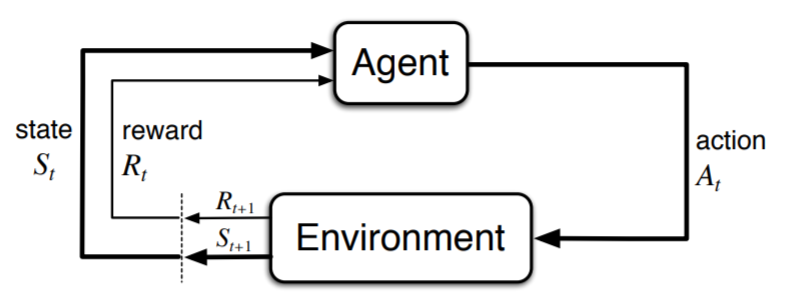
\includegraphics[width=\linewidth]{MDP_interface.PNG}
  \caption{The agent-environment interaction in a MDP}
  \label{fig:MDP_interface}
\end{figure}

At each time step $t$, the agent receives some representation of the environment's $state$, $S_t$, and on the state selects an $action$, $A_t$. One time step later, the agent receives reward $R_{t+1}$ as a result of the action, and find itself in a new state $S_{t+1}$. The trajectory/sequence is:

$$ S_0, A_0, R_1, S_1, A_1, R_2, S_2, A_2, R_3, \cdots $$

In a \textit{finite} MDP, the state sets, action sets and reward sets are finite.

Following defines the \textit{dynamics} of the MDP.

$$ p(s', r| s, a) \doteq P(S_t = s', R_t = r | S_{t-1} = s, A_{t-1} = a) $$
$$ \sum_{s' \in \mathcal{S}} \sum_{r \in \mathcal{R}} p(s',r|s,a) = 1, \forall s \in \mathcal{S}, a \in \mathcal{A}(s) $$

$p$ specifies a probability distribution for each choise of $s$ and $a$.
The probability of each possible value for $S_t$ and $R_t$ depends on the immediately preceding state and action, $S_{t-1}$ and $A_{t-1}$ (note not including earlier states and actions).

\begin{definition}
Markov property, a Markov state includes information about all aspects of the past agent-environment interaction, that make a difference for the future.
\end{definition}

\begin{definition}
state-transition probabilities,
$$ p(s'|s,a) \doteq P(S_t=s'|S_{t-1}=s, A_{t-1}=a) = \sum_{r\in \mathcal{R}} p(s',r|s,a) $$
\end{definition}

\begin{definition}
expected rewards for state-action pairs

$$ r(s,a) \doteq \E [R_t | S_{t-1}=s, A_{t-1}=a] = \sum_{r\in \mathcal{R}} \sum_{s\in \mathcal{S}} p(s',r|s,a) $$
\end{definition}

\begin{definition}
expected rewards for state-action-nextState,

$$ r(s,a,s') \doteq \E [R_t | S_{t-1}=s, A_{t-1}=a, S_t=s'] = \sum_{r \in \mathcal{R}} r \frac{p(s',r|s,a)}{p(s'|s,a)} $$
\end{definition}


\paragraph{agent-environment}
The agent-environment boundary represents the liit of the agent's absolute control, not of its knowledge. Anything that cannot be changed by the agent.

Any problem of learning goal-directed behavior can be reduced to 3 signals passing back and forth between an agent and its environment:
\begin{itemize}
\item action: the choicemade by the agent
\item the basis on which the choice is made
\item the agent's goal
\end{itemize}

\begin{example}
Bioreactor,

\begin{itemize}
\item actions (vector): target temperatures, target sitrring rates
\item states (vector): sensory readings, ingredients input, target chemical
\item rewards (number): production rate of useful chemical (target)
\end{itemize}

\end{example}

\begin{example}
Robotic Arm (pick-and-place task)

\begin{itemize}
\item actions: voltages applied to each joint motor
\item states: readings of joint angles and velocities
\item rewards: +1 for successfully object pick-and-place; small negative reward at each time step (punish jerkiness motion)
\end{itemize}
\end{example}


\subsection{Goals and Rewards}
 In RL, thr purpose/goal of the agent is to maximize \textit{cumulative reward in the long run}.
 It is important that the set-up rewards indicate what we truly want accomplished.
 In particular, rewards are not the place to tell/impart agent prior knowledge about \textit{how} to achieve our goal.
 For example, in a chess game, the agent should only be reward for winning, instead of achieving subgoals like taking oponent's pieces.
 Better places for imparting this kind of prior knowledge in (1) initial policy; or (2) initial value function.
 
 The reward signal is a way of imparting to the agent \textit{what} you want achieved, not \textit{how} you want it achieved.

\subsection{Returns and Episodes}

A RL agent's goal is to maximize the cumulative reward it receives in the long run.
In general, we seek to maximize the \textit{expected return} $G_t$.

$$ G_t \doteq R_{t+1} + R_{t+2} + \cdots + R_T $$

where $T$ is a final time step.

The final time step marks the end of a subsequences.

\begin{definition}
Episode, a subsequence of the agent-environment interaction. Each episode ends in \textbf{terminal state}, followed by a \textbf{reset} to a standard starting state or to a \textbf{sample} from a standard distribution of starting states. The next episode begins independently of how the previous one ended.
\end{definition}

The set of all nonterminal states, $\mathcal{S}$. All states and the terminal state, $\mathcal{S^+}$.

\begin{definition}
Episodic tasks, tasks with episodes that with terminal state.
\end{definition}

\begin{definition}
continuing tasks, tasks without terminal state.
\end{definition}

This task uses discounted rewards to deal with $T=\infty$.

\begin{definition}
discounted rewards $G_t$. discount rate, $0 \leq \gamma \leq 1$

$$ G_t \doteq R_{t+1} + \gamma R_{t+2} + \gamma^2 R_{t+3} + \cdots = \sum_{k=0}^{\infty} \gamma^k R_{t+k+1} $$
\end{definition}

The discount rate determines the present value of future rewards. As long as the reward sequence {$R_k$} is bounded, the infinite sum $G_t$ has a finite value.
If $\gamma \rightarrow 0$, the agent is myopic; if $\gamma \rightarrow 1$, the agent is farsighted.

If the reward is constant $R$, then we have the \textit{geometric series}

$$ G_t = \sum_{k=0}^{\infty} R\gamma^k = R\frac{1}{1-\gamma} $$

Note that the returns at successive time steps are related to each other (which is important for RL):

$$ G_t \doteq R_{t+1} + \gamma R_{t+2} + \gamma^2 R_{t+3} + \cdots = R_{t+1} + \gamma G_{t+1} $$

\begin{example} pole-balancing
\begin{itemize}
\item terimnal state: if the pole falls past a given angle from vertical or if the cart runs off the track
\item starting state: pole reset to vertical
\item reward (episodic): +1 for each time step before falling
\item reward (continuing): -1 on each falling, 0 for all other times
\end{itemize}
\end{example}


\begin{figure}[!h]
  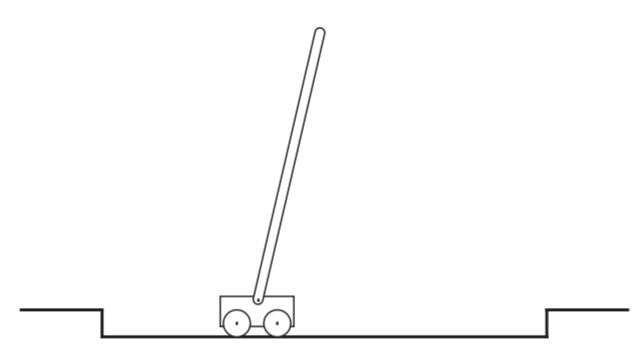
\includegraphics[width=\linewidth]{MDP_pole.PNG}
  \label{fig:MDP_pole}
\end{figure}



\subsection{Unified Notation for Episodic and Continuing Tasks}

We use $S_{t,i}$ to represents state at time $t$ of episode $i$ (same for $A_{t,i}$, $R_{t,i}$, etc).
In practice, we dropped the $i$ as we normally don't have to distinguish between different episodes.
So, now $S_t$ refers to $S_{t,i}$.

We use an $absorbing state$ to replace the terminate state. The absorbing state transits to itself and have reward = 0.
This way, we can have the same formula of $G_t$ for episodic and continuing tasks.

\subsection{Policies and Value Functions}

Value functions (either V or Q) are \textbf{always} conditional on some policy $\pi$. Sometimes in literature we leave off the $\pi$ or $*$ and just refer to $V$ and $Q$, because it’s implicit in the context, but ultimately, every value function is always with respect to some policies.

\begin{definition}
value functions of states, estimate how much expected return it is received for the agent to be in a given state
value functions of state-action pairs, estimate how much expected return it is received to perform a given action in a given state
\end{definition}

\begin{definition}
policy, $\pi(A_t=a|S_t=s)$, a mapping from states to probabilities of selecting each action
\end{definition}

Expectation of $R_{t+1}$ in terms of $\pi$ and the four-argument function $p$:
\[
\E\left[R_{t+1} \middle|S_{t}\right] = \sum_{a \in \mathcal{A}} \pi\left(a \middle| S_t\right) \cdot r(S_t, a) = \sum_{a \in \mathcal{A}} \pi\left(a \middle| S_t\right) \cdot \sum_{r \in \mathcal{R}} r \sum_{s' \in \mathcal{S}} p\left(s', r \middle| S_t, a\right)
\]
My word explanation: the expectation of reward given current state $S_t$= the total sum of the probability of perform action $a$ at state $s$ $\cdot$ the reward $r$ $\cdot$ the probability of getting reward $r$ (when performs action $a$ at state $s$) (?)

\begin{definition}
state-value function for policy $\pi$, (value function of a state $s$ under a policy $\pi$), $v_{\pi}(s)$, is the expected return when starting in $s$ and following $\pi$ thereafter. For MDPs:

$$ v_\pi(s) \doteq \E_\pi[G_t | S_t = s] = \E_\pi [ \sum_{k=0}^{\infty} \gamma^k R_{t+k+1} | S_t = s], \forall s \in \mathcal{S} $$
\end{definition}

\begin{definition}
action-value function for policy $\pi$, (value of taking action $a$ in state $s$ under a policy $\pi$), $q_\pi(s,a)$, as the expected return starting from $s$, taking the action $a$, and \textbf{then} following policy $\pi$:

$$ q_\pi(s,a) \doteq \E_\pi [G_t | S_t = s, A_t = a] = \E_\pi [\sum_{k=0}^{\infty} \gamma^k R_{t+k+1} | S_t = s, A_t = a] $$
\end{definition}

The main difference between $Q$ and $V$ then, is the $Q$-value lets you play a hypothetical of potentially taking a different action in the first time step than what the policy might prescribe and then following the policy from the state the agent winds up in.
\newline

Equation of $v_\pi$ in terms of $q_\pi$ and $\pi$:
$$ v_\pi(s) = \sum_a \pi(a|s)q_\pi(s,a) $$

My word explanation: the value function is the total sum of probability of choosing action $a$ at state $s$ $\times$ the action-value of taking each action.
\newline
Equation of $v_\pi$ in terms of $\pi$ and $p$:
\begin{align*}
v_\pi(s) & \doteq \E_\pi[G_t | S_t = s]\\
& = \E_\pi[R_{t+1} + \gamma G_{t+1} | S_t = s]\\
& = \sum_a \pi(a|s) \sum_{s'}\sum_r p(s',r|s,a) [r+ \gamma \E_\pi[G_{t+1} | S_{t+1}=s']]\\
& = \sum_a \pi(a|s) \sum_{s',r} p(s',r|s,a) [r+ \gamma v_\pi(s')]
\end{align*}

Equation of $q_\pi$ in terms of $v_\pi$ and the four argument $p$
$$ q_\pi(s,a) = \sum_{s', r} p(s',r|s,a) \underbrace{ [r+\gamma v_\pi(s')] }_{G_t?} $$

\begin{definition}
Monte Carlo methods, estimation methods that involve averaging over many random samples of actual returns.
\end{definition}

For example, an agent follows policy $\pi$; and for each state $s$, the agent maintains an average of the actual returns which have followed that state, then the average converges to the state's value $v_\pi(s)$. (Recall the Law of Large Numbers, or sample-average method in Chapter 2).
For another example, if separate averages are kept for each action taken in each state, then these averages will similarly converge to the action values $q_\pi(s,a)$.

\begin{definition}
Bellman equation for $v_\pi$:

$$ v_\pi = \sum_a \pi(a|s) \sum_{s',r} p(s',r|s,a) [r+ \gamma v_\pi(s')] $$
\end{definition}

It expresses a relationsihp between the value of a state and the values of its successor states.

\begin{figure}[!h]
  \centering
  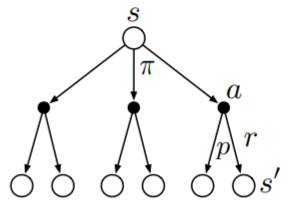
\includegraphics[]{MDP_backup.PNG}
  \caption{Backup diagram for $v_\pi$}
  \label{fig:MDP_backup}
\end{figure}
Note that in backup diagram, the nodes do not necessarily represent distinct states (e.g. a state might be its own successor).

The value function $v_\pi$ is the unique solution to its Bellman equation (??).

\begin{definition}
Bellman equation for $q_\pi$:

$$ q_\pi(s,a) \doteq \E_\pi [G_t | S_t = s, A_t = a] = \sum_{s',r} p(s',r|s,a)[r+\gamma \sum_{a'} \pi(a'|s')q_\pi (s',a')] $$
\end{definition}

\begin{figure}[!h]
  \centering
  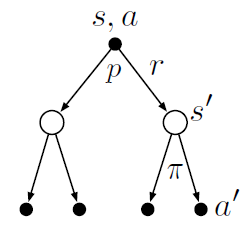
\includegraphics[]{MDP_backup_Qpi.PNG}
  \caption{Backup diagram for $q_\pi$}
  \label{fig:MDP_backup_qpi}
\end{figure}

\begin{figure}[!h]
    \centering
    \subfigure[]{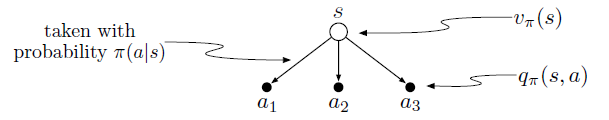
\includegraphics[width=\textwidth]{MDP_1.PNG}}
    \subfigure[]{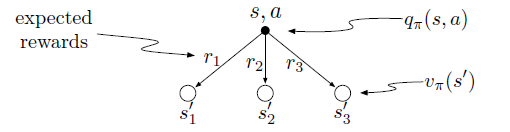
\includegraphics[width=\textwidth]{MDP_2.PNG}}
    \caption{ (a) $ v_\pi(s)=\sum_a \pi(a|s)q_\pi(s,a) $ (b) $ q_\pi(s,a)=\sum_{s',r}p(s',r|s,a)[r+\gamma v_\pi(s')] $ }
    \label{fig:MDPMDP}
\end{figure}
The value of a state depends on the values of the actions possible in that state and on how likely each action is to be taken under the current policy.

\subsection{Optimal Policies and Optimal Value Functions}

Solving a RL means finding a policy that achieves a lot of reward over the long run.

\begin{definition}
optimal policy, $\pi_*$

$$ \pi_* \geq \pi' \iff v_\pi(s) \geq v_{\pi'}(s), \quad \forall s \in \mathcal{S} $$
\end{definition}

\begin{definition}
optimal state-value function, $v_*$

$$ v_*(s) \doteq \max_\pi v_\pi(s), \quad \forall s \in \mathcal{S} $$
\end{definition}

\begin{definition}
optimal action-value function, $q_*$

$$ q_*(s) \doteq \max_\pi q_\pi(s,a), \quad \forall s \in \mathcal{s}, a \in \mathcal{A} $$
\end{definition}

We can write $q_*$ in terms of $v_*$:

$$ q_*(s,a) = \E [R_{t+1} + \gamma v_* (S_{t+1}) | S_t = s, A_t = a] $$

\begin{definition}
Bellman optimality equation for $v_*$,
\begin{align*}
v_*(s) & = \max_{a\in\mathcal{A}}(s) q_{\pi_*} (s,a) \\
& = \max_a \E [R_{t+1} + \gamma v_* (S_{t+1}) | S_t = s, A_t = a] \\
& = \max_a \sum_{s',r} p(s',r|s,a)[r+\gamma v_*(s')]
\end{align*}
\end{definition}

\begin{definition}
Bellman optimality equatoin for $q_*$,
\begin{align*}
q_*(s,a) & = \E [R_{t+1} + \gamma \max_{a'} q_*(S_{t+1}, a') | S_t = s, A_t = a] \\
& = \sum_{s',r} p(s',r|s,a)[r+\gamma \max_{a'} q_*(s',a')]
\end{align*}
\end{definition}

\begin{figure}[!h]
  \centering
  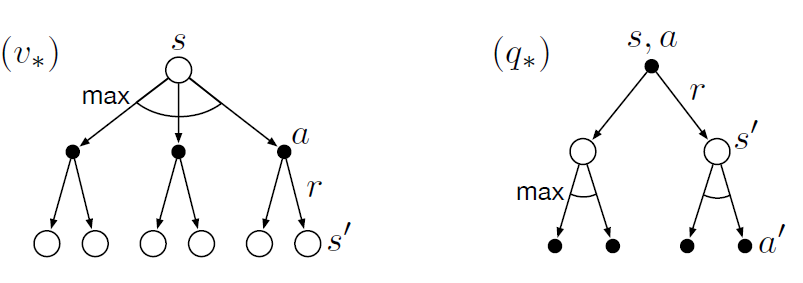
\includegraphics[]{MDP_optimal.PNG}
  \caption{Backup diagram for $v_*$ and $q_*$}
  \label{fig:MDP_optimal}
\end{figure}

Explicitly solving the Bellman optimality equation provides one route to finding $\pi_*$, and thus to solving the RL problem.
However, this solution is rarely useful. It needs an exhaustive search, looking ahead at all possibilities, computing their probabilities of occurrence and their desirabilities in terms of expected rewards.
This solution relies on at least 3 assumptions:
\begin{itemize}
\item the dynamics of the environment are accurately known
\item computational resources are sufficient
\item the states have the Markov property
\end{itemize}

In RL, one typically has to settle for approximate solutions. Many RL methods can be taken as approximately solving the Bellman optimality equation.

\paragraph{exercise} Consider the contining MDP shown, the only decision to be made is in the top state with two actions (left, right).
Find optimal policy when $\gamma$ = 0.9.

\begin{figure}[!h]
  \centering
  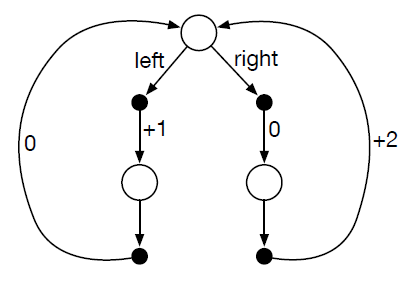
\includegraphics[]{ex3-22.PNG}
  \label{fig:ex3-22}
\end{figure}

Recall the definition of $v_\pi(s)$ and $q_\pi(s)$, we get

\begin{itemize}
\item Left Policy
\begin{itemize}
\item $ v(s_0) = 1 + 0.9\cdot v(s_L) $
\item $ v(s_L) = 0 + 0.9\cdot v(s_0) $
\item $ v(s_R) = 2 + 0.9\cdot v(s_0) $
\end{itemize}
\item Right Policy
\begin{itemize}
\item $ v(s_0) = 0 + 0.9\cdot v(s_R) $
\item $ v(s_L) = 0 + 0.9\cdot v(s_0) $
\item $ v(s_R) = 2 + 0.9\cdot v(s_0) $
\end{itemize}
\end{itemize}
Solving above we find that all state values of Right Policy is greater than all state values of Left Policy. Thus, `right' is the optimal policy for $\gamma$ = 0.9.

It is important to note that if we take `left' action in $s_0$, then policy $\pi$ would never take us to state $s_R$ (same for `right' and $s_L$); however, due to the definition of $\pi_*$, we must evaluate the value function for all states, even ones that would not be visited under a policy we are evaluating.

\subsection{Optimality and Approximation}

It is difficult to reach optimal solutions due to constraints from computational resource, memory. We can often approximate the optimal solutions.

\subsection{Summary}

\begin{itemize}
\item RL is about learning from interaction how to behave in order to achieve a goal.
\item RL \textit{agent} and its \textit{environment} interact over a sequence of discrete time steps.
\item \textit{actions}: choices made by the agent, \textit{states}: the basis for making the choices, \textit{rewards}: basis for evaluating the choices.
\item everything inside agent is known and controllable; environment is incompletely controllable, and are partialily known
\item a \textit{policy} is a stochastic rule that the agent selects actions as a function of states
\item agent's objective is to maximize reward it receives in the long run
\item when RL setup with agent, environment, states, actions, rewards, policy and formulated with well-defined transition probabilities it constitutes a Markov decision process (MDP)
\item a finite MDP is an MDP with finite state sets, action sets and reward sets.
\item \textit{return} is the function of future rewards that the agent seeks to maximize (in expected value)
\item undiscounted formulation is appropriate for \textit{episodic tasks}
\item discounted formulation is appropriate for \textit{tabular continuing tasks}
\item \textit{value functions} $v_\pi$ (state) and $q_\pi$ (state-action pair) are the expected return from that state/state-action under policy $\pi$
\item \textit{optimal value functions} $v_*$ and $q_*$ are the largest expected return by any policy
\item A policy whose value functions are optimal is an optimal policy
\item A MDP can have many optimal policies, but can have only one unique optimal value function ($v_*$ and $q_*$)
\item Any policy that is \textit{greedy} w.r.t $v_*$ and $q_*$ must be $\pi_*$
\item The Bellman optimality equations are special consistency conditions that the optimal value functions must satisfy
\item In RL most cases, their optimal solutions cannot be found but must be approximated in some way.
\end{itemize}

\section{Dynamic Programming}

In RL, DP refers to a collection of algorithms that can be used to compute optimal policies $\pi_*$ given a perfect model of the environment as a Markov decision process (MDP).
DP itself cannot be useful in RL due to its computational cost and requirement of a perfect model, but DP provides an essential foundation for the understanding of other algorithms.
Other algorithms can be treated as attempts to achieve much the same effect as DP, only with less computation and without assuming a perfect model of the environment.

Starting with this chapter, we assume the environment is a finite MDP (i.e. $S$, $A$, $R$ are finite and dynamics are given by a set of probabilities $p(s',r|s,a)$).
A common way of obtaining approximate solutions for tasks with continuous states and actions is to quantize the state and action spaces and then apply finite-state DP methods.
In this chapter we show how DP can be used to compute the value functions defined in Chapter 3. As shown in Chapter 3, we can obtain $\pi_*$ once we have found $v_*$ or $q_*$, which satisfy the Bellman optimality equations:

\begin{align*}
v_*(s) & = \max_a \E [R_{t+1} + \gamma v_*(S_{t+1}) | S_t = s, A_t = a] \\
& = \max_a \sum_{s',r} p(s',r|s,a)[r + \gamma v_*(s')]
\end{align*}

\begin{align*}
q_*(s,a) & = \E [R_{t+1} + \gamma \max_{a'} q_*(S_{t+1},a') | S_t = s, A_t = a] \\
& = \sum_{s',r} p(s',r|s,a)[r+\gamma \max_{a'} q_*(s',a')]
\end{align*}

\subsection{Policy Evaluation (Prediction)}
\begin{definition}
policy evaluation, compute the state-value function $v_\pi$ for an arbitrary policy $\pi$
\end{definition}

Policy evaluation is also called prediction problem.

Recall that $\forall s \in \mathcal{S}$,

\begin{align*}
v_\pi(s) & \doteq \E_\pi [G_t | S_t = s] \\
& = \E_\pi [R_{t+1} + \gamma G_{t+1} | S_t = s] \\
& = \E_\pi [R_{t+1} + \gamma v_\pi (S_{t+1}) | S_t = s] \\
& = \sum_a \pi (a|s) \sum_{s',r} p(s',r|s,a) [r+\gamma v_\pi (s')]
\end{align*}

If the environment's dynamics are completely known, then the last equation is a sysnteim of $|\mathcal{S}|$ simultaneous linear equations.
For this case, iterative solution methods are most suitable. Consider a sequence of approximate value functions $v_0$, $v_1$, $v_2$, $\cdots$, each mapping $\mathcal{S^+}$ to $\R$.
The initial approximation, $v_0$, is chosen arbitrarily, and each successive approximation is obtained by using the Bellman equation $v_\pi$ as an update rule ($\forall s$):

\begin{align*}
v_{k+1} & \doteq \E_\pi [R_{t+1} + \gamma v_k (S_{t+1}) | S_t = s] \\
& = \sum_a \pi (a|s) \sum_{s',r} p(s',r|s,a)[r+\gamma v_k (s')]
\end{align*}

We see that $v_k$ = $v_\pi$ is a fixed point for this update rule as $k \rightarrow \infty$, $v_k$ converages to $v_\pi$. This algorithm is called \textit{iterative policy evaluation}.
The update is called \textit{expected update}. It is called \textit{expected} because the updates are based on an expectation over all possible next states rather than on a sample next state.

In this algorithm, we use one array and update values in place.
\begin{tcolorbox}[width=\textwidth,title={Iterative Policy Evaluation, for estimating $V \approx v_\pi$}]
Input $\pi$ (the policy to be evaluated); $\theta > 0$ threshold determining accuracy of estimation.
Initialize $V(s)$ arbitrarily, for $s \in \mathcal{S}$, and $V$ to 0.

Loop:
\begin{align*}
&\quad\Delta \leftarrow 0 \\
&\quad\text{Loop for each } s \in \mathcal{S} \\
&\quad\quad v \leftarrow V(s) \\
&\quad\quad V(s) \leftarrow \sum_a \pi (a|s) \sum_{s',r} p(s',r|s,a)[r + \gamma V(s')] \\
&\quad\quad \Delta \leftarrow \text{max}(\Delta, |v-V(s)|) \\
&\text{until } \Delta < \theta
\end{align*}
\end{tcolorbox}


Policy evaluation of $q_\pi$:

\begin{align*}
q_\pi(s,a) & \doteq \E_\pi [G_t | S_t = s, A_t = a] \\
& = \E_\pi [R_{t+1} + \gamma G_{t+1} | S_t = s, A_t = a] \\
& = \E_\pi [R_{t+1} + \gamma \sum_{s',a'} q_\pi (s',a') | S_t = s, A_t = a] \\
& = \sum_{s',r} p(s',r|s,a) [ r+ \gamma \sum_{a'} \pi(a'|s')q_\pi(s',a')]
\end{align*}

\begin{align*}
q_{k+1}(s,a) & \doteq \E_\pi [R_{t+1} + \gamma G_{t+1} | S_t = s, A_t = a] \\
& = \sum_{s',r} p(s',r|s,a)[r+\gamma \sum_{a'} \pi (a'|s')q_k(s',a')]
\end{align*}

\subsection{Policy Improvement}

\begin{definition}
policy improvement theorem. Let $\pi$ and $\pi'$ be any pair of deterministic policies, where $\pi'$ is idential to $\pi$ except $\pi'(s) = a \neq \pi(s)$, s.t. $\forall s \in \mathcal{S}$,

$$ q_\pi (s,\pi'(s)) \geq v_\pi(s) $$

Then the policy $\pi'$ must be btter (or as good as) than $\pi$. That is, it must obtain greater or equal expected return from all states $s \in \mathcal{S}$

$$ v_{\pi'}(s) \geq v_\pi (s) $$
\end{definition}

\begin{definition}
policy improvement, the process of making a new policy $\pi'$ that improves on an original policy $\pi$, by making it greedy w.r.t the value function of $\pi$.
\end{definition}
 
If there are ties in policy improvement steps, each maximizing action can be given a portion of the probability of being selected in the new greedy policy.

\subsection{Policy Iteration}

It is trivial to see that we can ultimately reach an optimal policy through iterative improving policies and value functions \footnote{In large-scale reinforcement learning problems, it is typically impractical to run either of these steps to convergence, and instead the value function and policy are optimized jointly. By Soft Actor-Critic: Off-Policy Maximum Entropy Deep Reinforcement Learning with a Stochastic Actor}.

\begin{definition}
policy iteration, the way of finding an optimal policy.

$$\pi_0 \xrightarrow{E} v_{\pi_0} \xrightarrow{I} \pi' \xrightarrow{E} v_{\pi'} \xrightarrow{I} \pi'' \xrightarrow{E} \cdots \xrightarrow{I} \pi_* \xrightarrow{E} v_* $$
\end{definition}

\begin{tcolorbox}[width=\textwidth,title={Policy Iteration (using iterative policy evaluation) for estimating $\pi \approx \pi_*$}]
1. Initialization

$\quad V(s) \in\R$ and $\pi(s) \in A(s)$ arbitrarily $\forall s \in \mathcal{S}$; $V(terminal) \doteq 0$

2. Policy Evaluation
\begin{align*}
&\text{Loop:}\\
&\quad\Delta \leftarrow 0\\
&\quad\text{Loop for each } s \in \mathcal{S}\\
&\quad\quad v \leftarrow V(s)\\
&\quad\quad V(s) \leftarrow \sum_a \pi (a|s) \sum_{s',r} p(s',r|s,a)[r + \gamma V(s')]\\
&\quad\quad \Delta \leftarrow \text{max}(\Delta, |v-V(s)|)\\
&\text{until } \Delta < \theta
\end{align*}

3. Policy Improvement
\begin{align*}
&policyStable \leftarrow true\\
&\text{For each } s \in \mathcal{S}\\
&\quad oldAction \leftarrow \pi(s)\\
&\quad \pi(s) \leftarrow \argmax_a \sum_{s',r} p(s',r|s,a)[r+\gamma V(s')]\\
&\quad \text{If } oldAction \notin \{a_i\} \text{, which is the all equal best solutions from $\pi(s)$}\\
& \quad \text{then } policyStable \leftarrow false\\
&\text{If } policyStable \text{, then stop and return } V \approx v_* \text{ and } \pi \approx \pi_*\text{; else go to 2}	
\end{align*}
\end{tcolorbox}

\begin{tcolorbox}[width=\textwidth,title={Policy Iteration (using iterative policy evaluation) for estimating $\pi \approx \pi_*$}]
1. Initialization

$\quad Q(s,a) \in\R$ and $\pi(s) \in A(s)$ arbitrarily $\forall s \in \mathcal{S}, a \in \mathcal{A}$

2. Policy Evaluation
\begin{align*}
&\text{Loop:}\\
&\quad\Delta \leftarrow 0\\
&\quad\text{Loop for each } s \in \mathcal{S}, a \in \mathcal{A}\\
&\quad\quad q \leftarrow Q(s,a)\\
&\quad\quad Q(s,a) \leftarrow \sum_{s',r} p(s',r|s,a)[r + \gamma \sum_{a'}\pi(a'|s')Q(s',a')]\\
&\quad\quad \Delta \leftarrow \text{max}(\Delta, |q-Q(s,a)|)\\
&\text{until } \Delta < \theta
\end{align*}

3. Policy Improvement
\begin{align*}
&policyStable \leftarrow true\\
&\text{For each } s \in \mathcal{S}, a \in \mathcal{A}\\
&\quad oldAction \leftarrow \pi(s)\\
&\quad \pi(s) \leftarrow \argmax_a Q(s,a)\\
&\quad \text{If } oldAction \notin \{a_i\} \text{, which is the all equal best solutions from $\pi(s)$}\\
& \quad \text{then } policyStable \leftarrow false\\
&\text{If } policyStable \text{, then stop and return } Q \approx q_* \text{ and } \pi \approx \pi_*\text{; else go to 2}	
\end{align*}
\end{tcolorbox}


\begin{definition}
$\varepsilon$-soft, the probability of selecting each action in each state, is at least $\frac{\varepsilon}{A(s)}$
\end{definition}

\subsection{Value Iteration}

The policy evaluation of policy iteration requires multiple sweeps through the state set and convergence occurs only in the limit.
We want to truncate policy evaluation without losing the convergence guarantees of policy iteration. One of the technique is value iteration.

\begin{definition}
value iteration, stop policy evaluation after one sweep (one update after each state).

\begin{align*}
v_{k+1}(s) & \doteq max_a \E [R_{t+1}+\gamma v_k(S_{t+1})|S_t = s, A_t = a]\\
& = max_a \sum_{s',r} p(s',r|s,a)[r+\gamma v_k (s')], \forall s \in \mathcal{S}
\end{align*}
\end{definition}










\newpage
\section{Some Notes}


% Please add the following required packages to your document preamble:
\begin{table}[]
\begin{tabular}{@{}ll@{}}
\toprule
on-policy                       & off-policy                                                                                                                  \\ \midrule
Agent can pick actions          & Agent can't pick actions                                                                                                    \\
most obvious setup :)           & \begin{tabular}[c]{@{}l@{}}learning with exploration\\ playing without exploration\end{tabular}                             \\
Agent always follows own policy & \begin{tabular}[c]{@{}l@{}}Learning from expert (expert is imperfect)\\ Learning from sessions (recorded data)\end{tabular} \\ \bottomrule
\end{tabular}
\end{table}

% Please add the following required packages to your document preamble:
% \usepackage{booktabs}
\begin{table}[]
\begin{tabular}{@{}lll@{}}
\toprule
             & on-policy                                                                                                                                   & off-policy                                                                          \\ \midrule
value based  & \begin{tabular}[c]{@{}l@{}}Monte Carlo Learning\\ TD(0)\\ SARSA\\ Expected SARSA\\ n-Step TD/SARSA\\ TD(\textbackslash{}lamda)\end{tabular} & \begin{tabular}[c]{@{}l@{}}Q-Learning\\ DQN\\ Double DQN\\ Dueling DQN\end{tabular} \\
policy based & \begin{tabular}[c]{@{}l@{}}REINFORCE\\ REINFORCE with Advantage\end{tabular}                                                                &                                                                                     \\
actor-critic & \begin{tabular}[c]{@{}l@{}}A3C\\ A2C\\ TRPO\\ PPO\end{tabular}                                                                              & \begin{tabular}[c]{@{}l@{}}DDPG\\ TD3\\ SAC\\ IMPALA\end{tabular}                   \\ \bottomrule
\end{tabular}
\end{table}


\subsection{Gradient Descent vs. Gradient Ascent}

The gradient of a continuous function $f$ = the vector that contains the partial derivatives $\frac{\partial f(p)}{\partial x_i}$ computed at that point $p$.
The gradient is finite and defined if and only if all partial derivatives are also defined and finite.
The gradient formula:

$$ \nabla f(x) = [\frac{\partial f(p)}{\partial x_1}, \frac{\partial f(p)}{\partial x_2}, \cdots, \frac{\partial f(p)}{\partial x_{|x|}}]^T $$

When using the gradient for optimization, we can either conduct gradient descent or gradient ascent.

\paragraph{Gradient Descent}
Gradient Descent is an iterative process through which we optimize the parameters of a ML model. It's particularly used in NN, but also in logistic regression and support vector machines (SVM). It is the most typical method for iterative minimization of a cost function. Its major limitation consists of its guaranteed convergence to a local, not necesarily global, minimum.

A hyperparameter (i.e. pre-defined parameter) $\alpha$ (learning rate), allows the fine-tuning of the process of decent. In particular, we may descent to a global minimum.
The gradient is calculated with respect to a vector of parameters for the model, typically the weight $w$. In NN, the process of applying gradient descent to the weight matrix is called backpropagation of the error.

Backpropagation uses the sign of the gradient to determine whether the weights should increase or decrease. The sign of the gradient allows us to direction of the closet minimum to the cost function. For a given $\alpha$, we iteratively optimize the vector $w$ by computing
$$ w_{n+1} = w_n - \alpha \nabla_w f(w) $$
At step $n$, the weights of the NN are all modified by the product of the hyperparameter $\alpha$ times the gradient of the cost function, computed with those weights.
If the gradient is positive, then we decrease the weights; if the gradient is negative, then we increase the weights.

\paragraph{Gradient Ascent}
Gradient ascent works in the same manner as gradient descent. The only difference is that gradient ascent maximize functions (instead of minimization).
$$ w_{n+1} = w_n + \alpha \nabla_w f(w) $$

Gradient descent works on \textbf{convex functions}, while gradient ascent works on \textbf{concave functions}.

\paragraph{Summary}
\begin{itemize}
\item The gradient is the vector containing all partial derivatives of a function in a point
\item We can apply gradient descent on a convex function, and gradient ascent on a concave function
\item Gradient descent finds the nearest minimum of a function, gradient ascent finds the nearest maximum
\item We can use either form of optimization for the same problem if we can flip the objective function.
\end{itemize}

\paragraph{Gradient vs. Derivative}

\begin{itemize}
\item A directional derivative = a slope in an arbitrary specified direction.
\item A directional derivative is a rate of change of a function in any given direction.
\end{itemize}

\begin{itemize}
\item Gradient = a vector with slope of the function along each of the coordinate axes.
\item Gradient indicates the direction of \textbf{greatest} change of a funciton of more than one variable.
\item Gradient vector can be interpreted as the `direction and rate of fastest increase'.
\end{itemize}

\paragraph{Differential vs. Derivative}
\begin{itemize}
\item Differential is a subfield of calculus that refers to infinitesimal difference in some varying quantity
\item Differential represents an equation that contains a function and one or more derivatives of that function
\item The function which represents the relationsihp between the dependent and the independent variables is unknown
\end{itemize}

\begin{itemize}
\item The derivative of a function is the rate of change of the output value with respect to its input value
\item Derivative represent the instantaneous change in the dependent variable with respect to its independent variable
\item The function which represents the relationship between the variables is known
\end{itemize}


\paragraph{Loss/Cost/Objective function}

\begin{itemize}
\item \textbf{Loss function} is usually a function defined on a data point, prediction and label, and measures the penalty. For example: square loss in linear regression, hinge loss in SVM, 01 loss in theoretical analysis
\item \textbf{Cost function} is usually more general. It might be a sum of loss functions over all training set plus some model complexity penalty. For example: MSE and SVM cost function
\item \textbf{Objective function} is the most general term for any function that you optimize during training. For example, a probability of generating training set in maximum likelihood approach is a well defined objective function, but it is not a loss function nor cost function
\end{itemize}

We may say that, a loss function is a part of cost function which is a type of an objective function.

From wikipedia, in mathematical optimization and decision theory, a loss function or cost function (sometimes also called an error function) is a function that maps an event or values of one or more variables onto a real number intuitively representing some "cost" associated with the event. An optimization problem seeks to minimize a loss function. An objective function is either a loss function or its opposite (in specific domains, variously called a reward function, a profit function, a utility function, a fitness function, etc.), in which case it is to be maximized.

\paragraph{Surrogate vs. Approximation}

I think surrogate and approximation can be used interchangeably.

Surrogate loss function is used when the original loss function is inconvenient for calculation.


\bibliography{references.bib}

\end{document}
















